\section{Introduction}

Database Management Systems are complex software systems, that are a result of decades of research and software development work in academia and industry.
They are at the core of many of the software applications.
Out of the many types of database management systems, relational database management systems remains the most widely used type.
Apart from being widely used, they have also influenced much of the development of other popular data management systems such as NoSQL, Big Data, and Machine Learning Systems.
Thus for this paper, we primarily focus on relational database management systems.

Machine learning is a sub-field of artificial intelligence that focuses on enabling software systems to perform tasks by learning from data or experience without being explicitly programmed.


% \begin{figure}
% 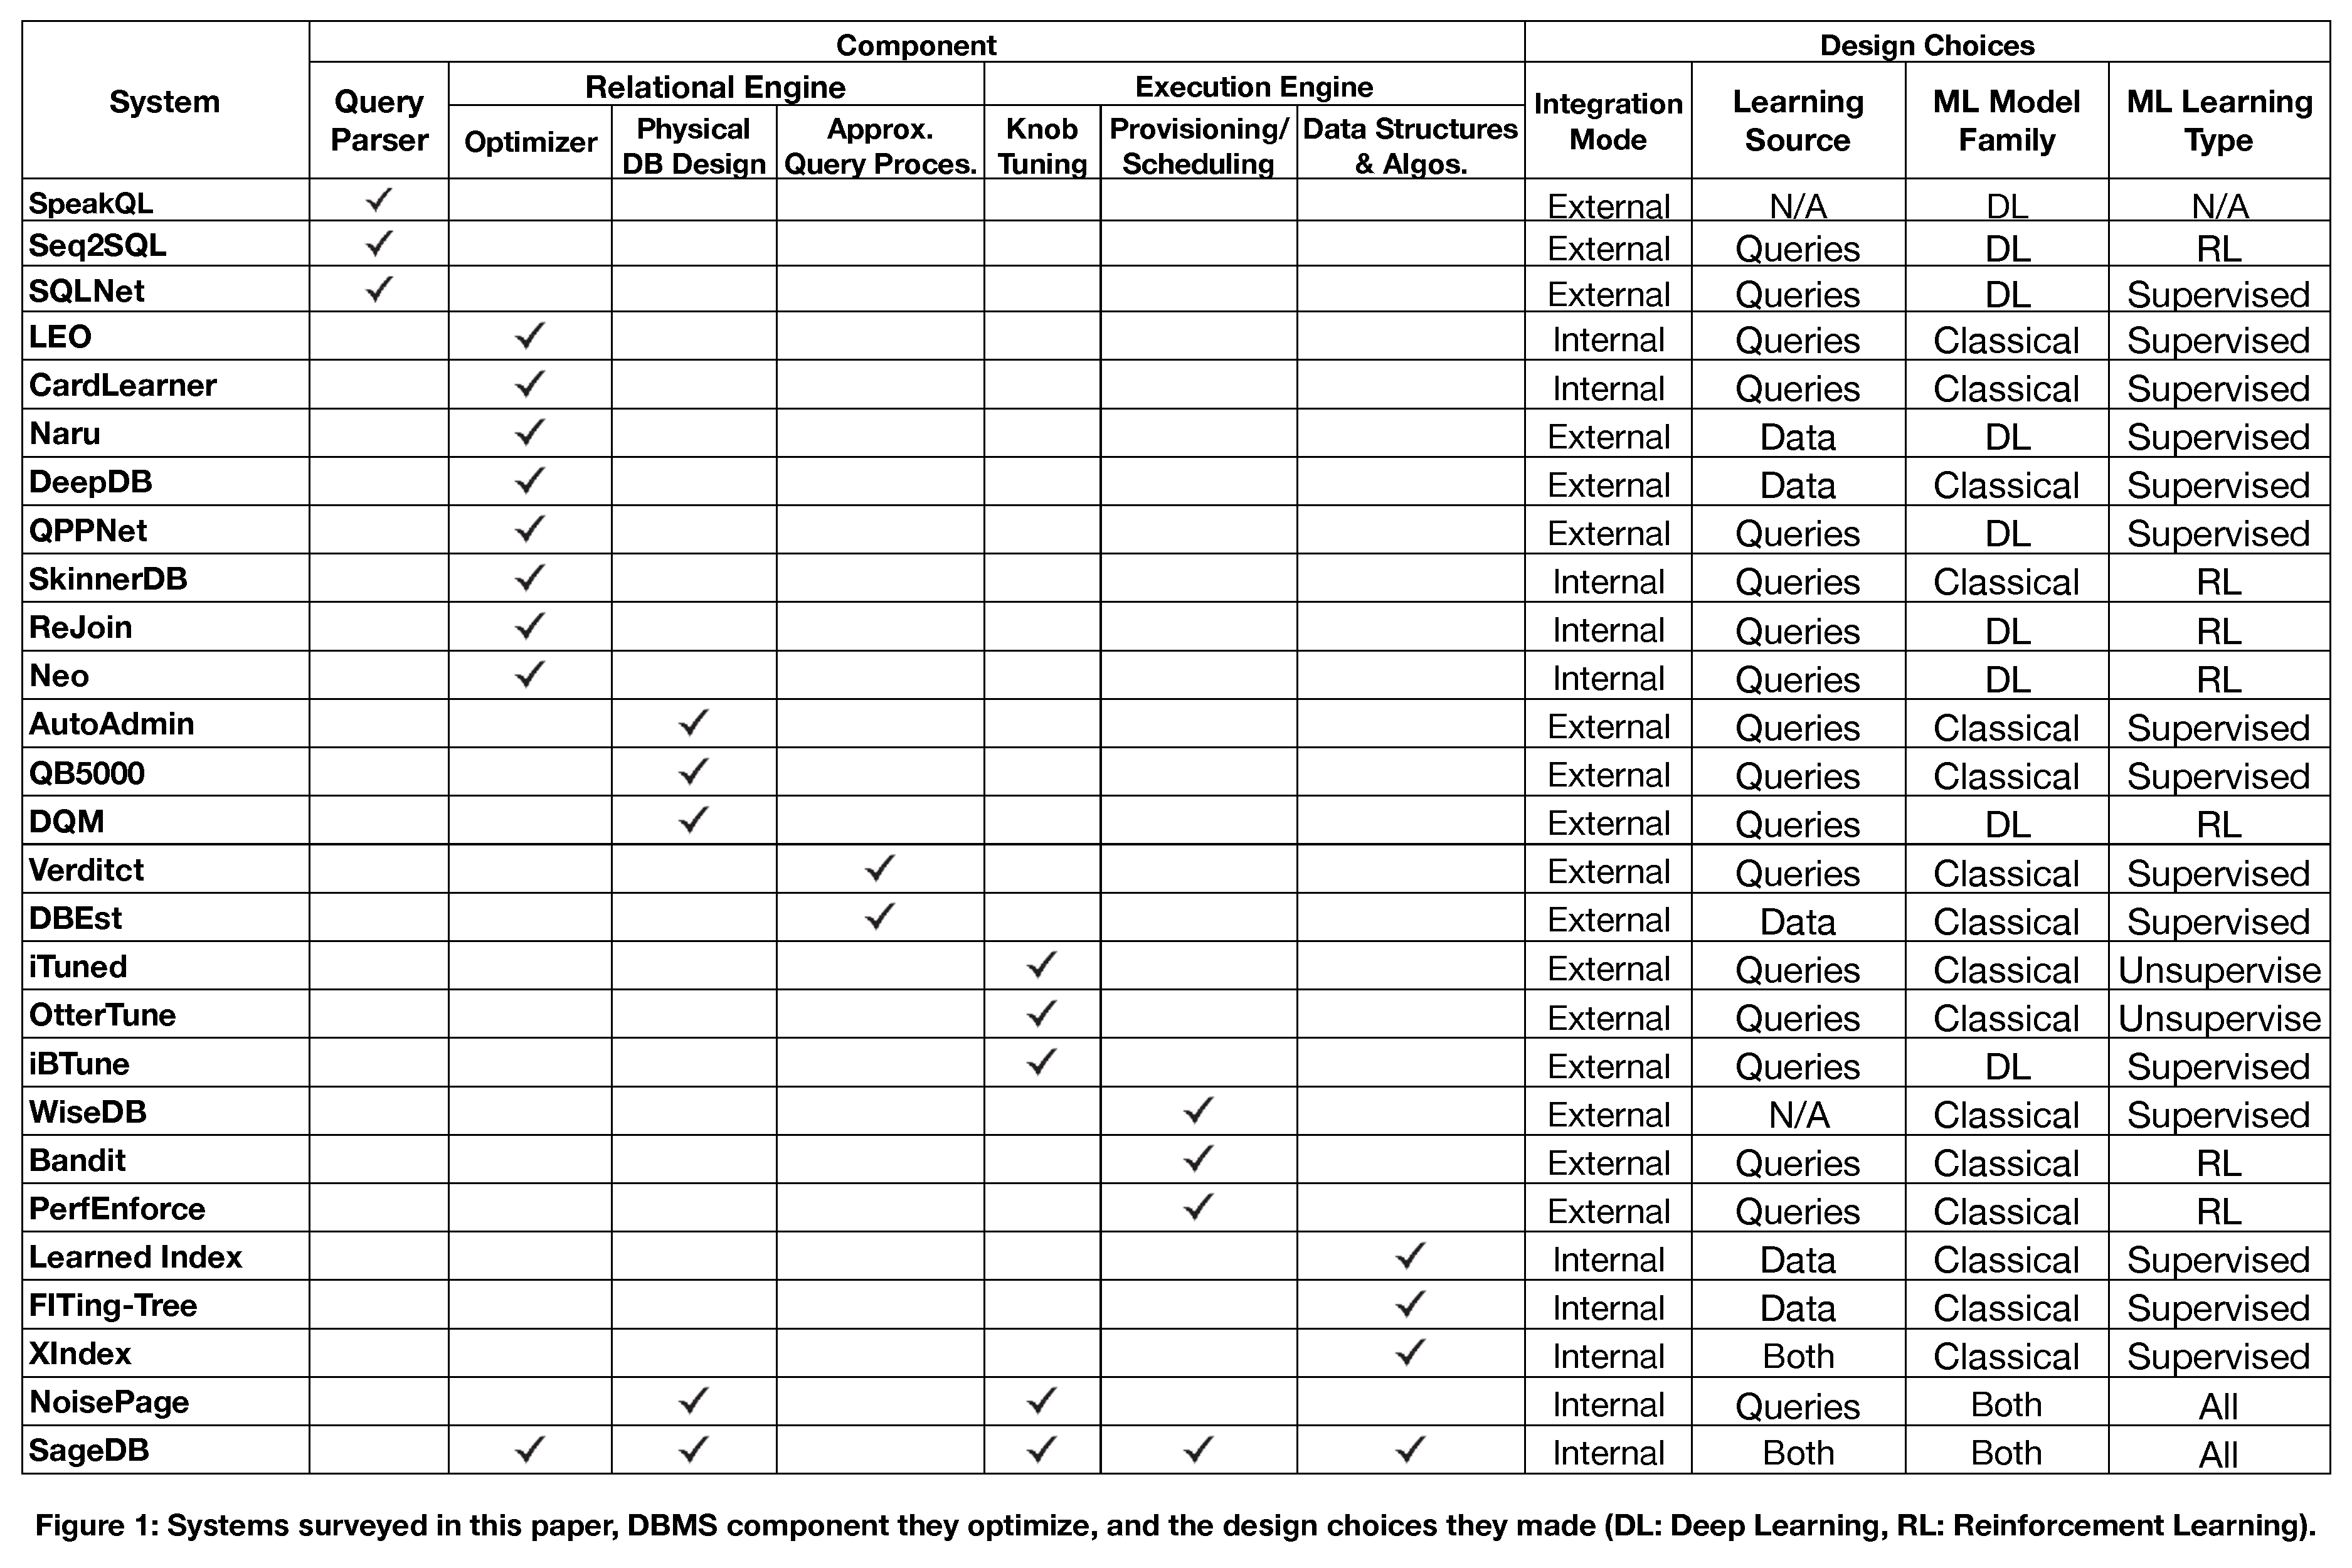
\includegraphics[width=\textwidth]{images/taxonomy.pdf}
% \end{figure}